\documentclass[aspectratio=169]{beamer}

% Thème
\usetheme{Marburg}

% Packages
\usepackage{lmodern}
\usepackage{amsfonts, amsmath, amssymb, mathrsfs}
\usepackage{enumitem}
\usepackage{graphicx}
\usepackage{pdfpages}
\usepackage{caption, subcaption}

% Barre Pied de page
\setbeamertemplate{footline}{
  \begin{beamercolorbox}[wd=\paperwidth,ht=2.25ex,dp=1ex]{author in head/foot}
    \usebeamerfont{author in head/foot}
    \hspace*{2ex}\insertauthor \hfill \inserttitle \hfill \insertdate \hfill \insertframenumber/\inserttotalframenumber\hspace*{2ex}
  \end{beamercolorbox}
}

% Barre de navigation
\setbeamertemplate{subsection in sidebar shaded}{}
\setbeamertemplate{title in sidebar shaded}{}
\setbeamertemplate{author in sidebar shaded}{}

% Barre d'en tête
\setbeamertemplate{headline}[CambridgeUS]


% Titre
\title{Forum MP2I-MPI 2024}
\author{Étudiants de MP2I-MPI}
\date{24 fevrier 2024}

\begin{document}

\begin{frame}
  \titlepage
\end{frame}

%TODO: Ajouter planing forum

\section{Planing du forum 2024 des MP2I-MPI}

\begin{frame}
    \begin{figure}
        \centering
        
\includegraphics[width=0.9\textwidth]{ressource_diapo/place older.png}
        \caption{Planing du forum 2024 des MP2I-MPI}
    \end{figure}
\end{frame}

\section{statistiques}

\subsection{Resultats Parcoursup}

\begin{frame}
    \begin{figure}
        \centering
        
\includegraphics[width=0.9\textwidth]{ressource_diapo/place older.png}
        \caption{Resultats Parcoursup}
    \end{figure}
\end{frame}

\subsection{Statistiques des mentions}

\begin{frame}
    \begin{figure}
        \centering
        
\includegraphics[width=0.9\textwidth]{ressource_diapo/place older.png}
        \caption{Statistiques des mentions}
    \end{figure}
\end{frame}

\subsection{admission en école d'ingénieur}

\begin{frame}
    \begin{figure}
        \centering
        
\includegraphics[width=0.9\textwidth]{ressource_diapo/place older.png}
        \caption{admission en école d'ingénieur}
    \end{figure}
\end{frame}

\section{Différentes filières}

\subsection{Répartition horaire}

\begin{frame}
    \begin{figure}
        \centering
        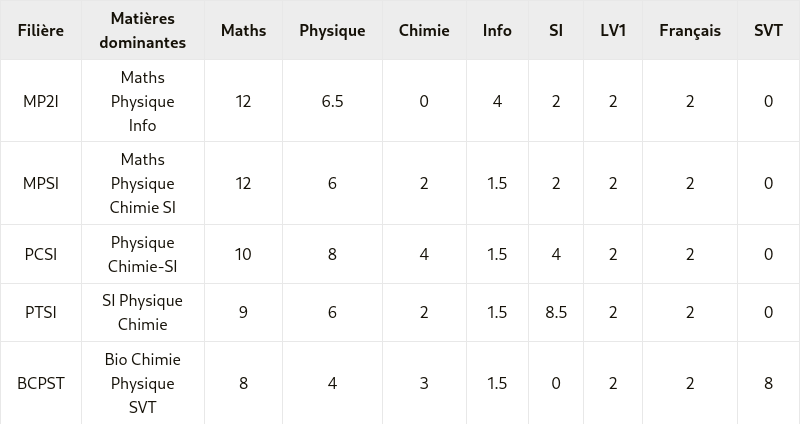
\includegraphics[width=\textwidth]{ressource_diapo/prepas.png}
        \caption{Répartition horaire}
    \end{figure}
\end{frame}

\subsection{Passage en deuxième année}

\begin{frame}
    \begin{figure}
        \centering
        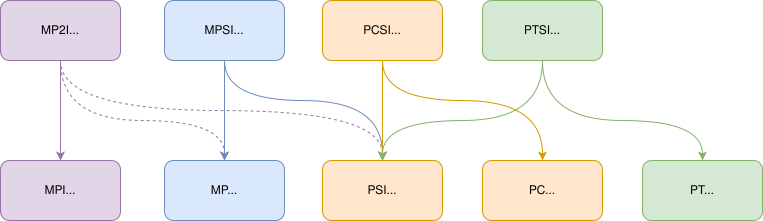
\includegraphics[width=\textwidth]{ressource_diapo/deuxieme_annee.png}
        \caption{Passage en deuxième année}
    \end{figure}
\end{frame}

\section{Vie en prépas}

\subsection{L'internat}

\begin{frame}
    \begin{figure}
        \centering
        
\includegraphics[width=0.9\textwidth]{ressource_diapo/place older.png}
        \caption{L'internat}
    \end{figure}
\end{frame}

\subsection{emploi du temps}

\begin{frame}
    \begin{figure}
        \centering
        
\includegraphics[width=0.9\textwidth]{ressource_diapo/place older.png}
        \caption{emploi du temps}
    \end{figure}
\end{frame}

\subsection{repartition aux concours}

\begin{frame}
    \begin{figure}[h]
        \begin{subfigure}{0.49\textwidth}
            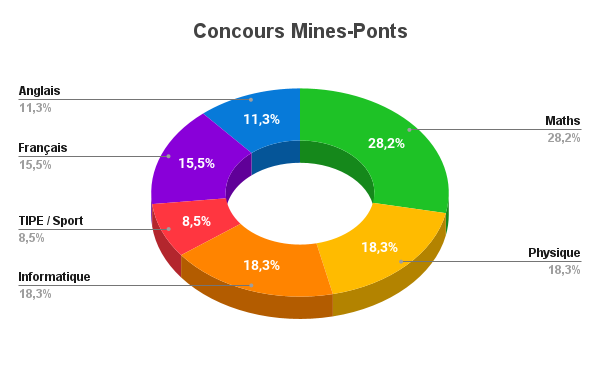
\includegraphics[width=0.95\linewidth]{ressource_diapo/Mines-Ponts.png}
        \end{subfigure}
        \begin{subfigure}{0.49\textwidth}
            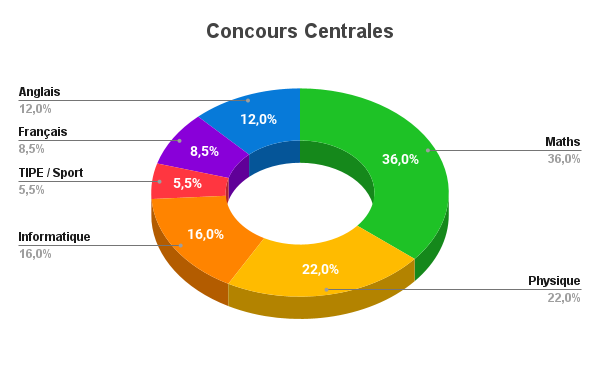
\includegraphics[width=0.95\linewidth]{ressource_diapo/Centrales.png}
        \end{subfigure}
        \begin{subfigure}{0.49\textwidth}
            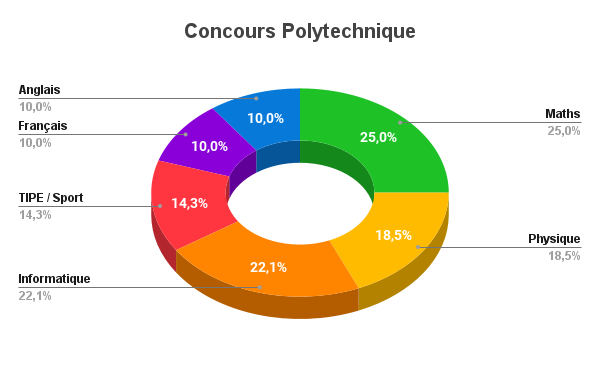
\includegraphics[width=0.95\linewidth]{ressource_diapo/X.png}
        \end{subfigure}
        \begin{subfigure}{0.49\textwidth}
            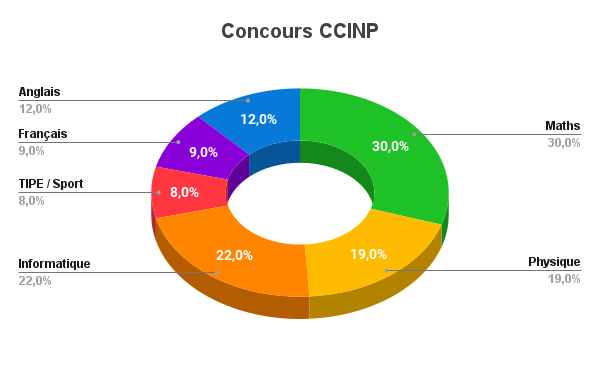
\includegraphics[width=0.95\linewidth]{ressource_diapo/CCINP.png}
        \end{subfigure}
    \end{figure}
\end{frame}

\section{Mathématiques}

\subsection{programme officiel}

\begin{frame}
    \begin{figure}
        \centering
        
\includegraphics[width=0.9\textwidth]{ressource_diapo/place older.png}
        \caption{programme officiel}
    \end{figure}
\end{frame}

\section{Physique}

\subsection{programme officiel}

\begin{frame}
    \begin{figure}
        \centering
        
\includegraphics[width=0.9\textwidth]{ressource_diapo/place older.png}
        \caption{programme officiel}
    \end{figure}
\end{frame}

\section{Informatique}

\subsection{programme officiel}

\begin{frame}
    \begin{figure}
        \centering
        
\includegraphics[width=0.9\textwidth]{ressource_diapo/place older.png}
        \caption{programme officiel}
    \end{figure}
\end{frame}

\subsection{Langage : OcamL}

\begin{frame}
    \begin{figure}
        \centering
        
\includegraphics[width=0.9\textwidth]{ressource_diapo/place older.png}
        \caption{OcamL}
    \end{figure}
\end{frame}

\subsection{Langage : C}

\begin{frame}
    \begin{figure}
        \centering
        
\includegraphics[width=0.9\textwidth]{ressource_diapo/place older.png}
        \caption{C}
    \end{figure}
\end{frame}

\subsection{Premier semestre}

\begin{frame}
    \begin{figure}
        \centering
        
\includegraphics[width=0.9\textwidth]{ressource_diapo/place older.png}
        \caption{Premier semestre}
    \end{figure}
\end{frame}

\subsection{Deuxième semestre}

\begin{frame}
    \begin{figure}
        \centering
        
\includegraphics[width=0.9\textwidth]{ressource_diapo/place older.png}
        \caption{Deuxième semestre}
    \end{figure}
\end{frame}

\section{conseils}

\subsection{avant la prépa}

\begin{frame}
    \begin{figure}
        \centering
        
\includegraphics[width=0.9\textwidth]{ressource_diapo/place older.png}
        \caption{avant la prépa}
    \end{figure}
\end{frame}

\subsection{pendant la prépa}

\begin{frame}
    \begin{figure}
        \centering
        
\includegraphics[width=0.9\textwidth]{ressource_diapo/place older.png}
        \caption{pendant la prépa}
    \end{figure}
\end{frame}

\section{FAQ}

\begin{frame}
    Exemple de question :

    \begin{itemize}
        \item Comment se passe la vie en prépa ?
        \item Quels sont les débouchés après une prépa ?
        \item Comment se passe les concours ?
        \item Quels sont les matières enseignées ?
        \item Comment se passe la vie en internat ?
    \end{itemize}
\end{frame}

\section{Annexe}

\begin{frame}
    \begin{figure}
        \centering
        
\includegraphics[width=0.35\textwidth]{ressource_diapo/logo_discord.png}
    \end{figure}
    \textbf{Notre discord :} \textit{https://discord.gg/Mu439mBdsv}\\
    \textbf{Notre site :} \textit{https://prepas-mp2i.fr}
\end{frame}

\end{document}
